


\begin{figure*}[h!]
\begin{center}
   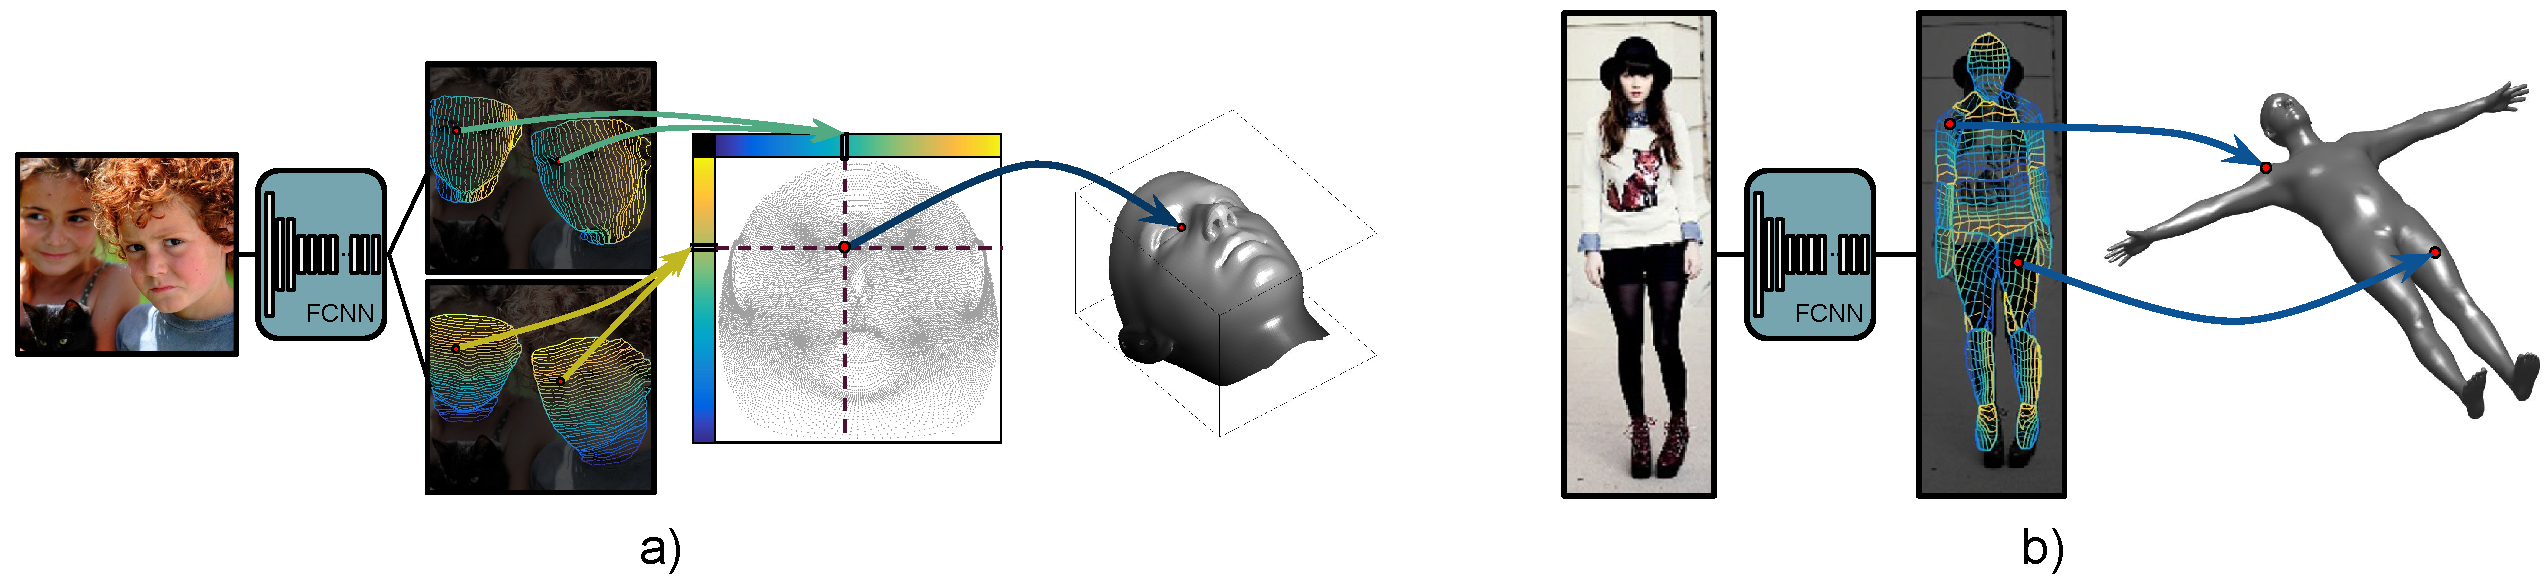
\includegraphics[width=1\linewidth]{Figures/denseregPami2}
\end{center}
   \caption{ We introduce a fully convolutional neural network that regresses from the image to a ``canonical'', deformation-free parameterization of the shape surface, effectively yielding a dense 2D-to-3D surface correspondence field. The system is depicted for dense correspondence between template shapes of \textit{a):} human face \textit{b):} human body.}
\label{fig:intro}
\end{figure*}


Deep Convolutional Neural Networks CNNs \citep{lecun1998gradient}
have revolutionized computer vision over the last decade, starting from  image classification \citep{krizhevsky2012imagenet, simonyan2014very, szegedy2015going,he2016deep}, and then moving on to tasks such as object detection \citep{girshick2014rich}, semantic segmentation \citep{long2015fully,chen2016deeplab} and pose estimation \citep{chen2014articulated, tompson2014joint,yang2016end,newell2016stacked}.
The order in which these tasks were successfully tackled can  be associated with the level of spatial detail at which the problem is addressed, starting from boxes, moving on to regions, and eventually getting to the  pixel-level labelling.

In this work we push further the envelope of tasks that can be addressed by CNNs, and consider a task that lies at the end of the `location detail' spectrum.
 Rather than characterizing  the region, or a few select points  that relate to an object, we aim at establishing a dense correspondence between 2D  and 3D surface coordinates, where the surface represents a template (or atlas) for a visual category, such as the human face or body. 
We show that  this task can be successfully addressed in an entirely feedforward manner by employing a discriminatively-trained CNN. 

%capture all of the excruciating details underlying image-to-model matching
%tackle the much more challenging task of establishing a 2D to 3D correspondence {\emph{in the wild}} by leveraging upon recent advances in semantic segmentation \citep{CP2015Semantic}. 
%one of the most `exchaustively detailed' visual tasks, namely  dense image-to-surface correspondence `in the wild',  
%semantic segmentation fine-grained categorization \citep{zhang2014part}, among others.
%Motivated by the gap between discriminatively trained systems for detection and category-level deformable models, we propose a system that combines the merits of both.
%Discriminative learning-based approaches typically pursue invariance to shape deformations, for instance by employing  local `max-pooling' operations to ellicit responses that are invariant to {\emph{local}} translations. As such, these models can reliably  detect patterns irrespective of their deformations through efficient, feedforward algorithms. At the same time, however, this discards useful shape-related information and only delivers a single categorical decision per position. 
%We introduce a discriminatively trained network to obtain, in a fully-convolutional manner, dense correspondences between an input image and a deformation-free template coordinate system. 

In order to accomplish this 
 we exploit the availability of manual landmark annotations ``in-the-wild'' in order to fit a 3D template; this provides us with a dense correspondence field, from the image domain to the 2-dimensional, $U-V$ parameterization of the surface. We then train a fully convolutional network that densely regresses from the image pixels to this $U-V$ coordinate space. This combines the fine-grained discrimative power of statistical deformable models with the ``in the wild'' operation of fully-convolutional neural networks. 
 We draw inspiration from recent successes of object detection at the task of bounding box regression \citep{ren2015faster}, and 
 introduce a method that blends classification and regression to accurately regress the 2D template coordinates of every foreground pixel.
 
 As we show experimentally, the proposed  feedforward architecture outperforms substantially more involved systems developped in particular for facial landmark localization while also outperforming the results of systems trained on lower-granularity tasks, such as facial part segmentation.
We can also seamlessly integrate this method with iterative, deformable model-based algorithms to obtain results that constitute the current state-of-the-art on large-scale, challenging facial landmark localization benchmarks.

%This provides us with dense and fine-grained correspondence information, as in the case of SDMs, while at the same time being independent of any initialization procedure, as in the case of discriminatively trained `fully-convolutional' networks. 


Furthermore, we show that by exploiting the established dense shape correspondence one can substantially improve the performance of CNNs trained for articulated body pose estimation and facial landmark localization and accelerate their training. 
In particular, recent CNN-based body and facial pose estimation works  only implicitly capture shape-based e.g. through cascading \citep{newell2016stacked}.  Instead, we further exploit shape for CNN  training by introducing an auxiliary dense correspondence supervision signal that acts like a source  of  `Privileged Information' \citep{VapnikV09,lopez2015unifying,ChenJFY17}.
Our experiments show that the cascading and dense supervision approaches are clearly complementary and can be combined, yielding faster and improved convergence. 

%\footnote{`Privileged Information' was proposed in \citep{VapnikV09} where it is argued that one can simplify training through the use of an `Intelligent Teacher' that in a way explains the supervision signal, rather than simply penalising misclassifications. This technique was recently used in deep learning for the task of image classification \citep{ChenJFY17}.}.

%We note that  this additional information is only available during training,  only serves as a means of simplifying the training problem, and only requires landmark-level annotations, as all current methods do.

%%%%%%%%%%%%%%%%%%%%%%%%%%%%%%%%%%%%%%%%

We can summarize our contributions as follows:
\begin{itemize}
\item We introduce the task of dense shape regression in the setting of CNNs, and exploit the notion of a deformation-free UV-space to construct target ground-truth signals (Sec.\ref{sec:SDMs}).
\item We propose a carefully-designed fully-convolutional shape regression system that exploits ideas from semantic segmentation and dense regression networks. Our \textit{quantized regression} architecture~(Sec.\ref{sec:quantized}) is shown to substantially outperform simpler baselines that consider the task as a plain regression problem. 
\item We use dense shape regression to jointly tackle a multitude of problems, such as landmark localization or semantic segmentation.
In particular, the template coordinates allow us to transfer to an image multiple annotations constructed on a single template system, and thereby tackle multiple problems through a single network.
\item We use the regressed shape coordinates for the initialization of statistical deformable models; systematic evaluations on facial analysis benchmarks show that this yields substantial performance improvements  on tasks.
\item We  show that a cascaded architecture that jointly regresses dense correspondences and sparse landmarks leads to improved localization in both articulated body pose estimation and facial landmark localization. 
\item We  demonstrate the generic nature of the method by applying it to the task of estimating dense correspondence in other object, such as the human ear.
\end{itemize}
A preliminary version of the paper has appeared in CVPR 2017 \citep{guler2016densereg}. The present version bears substantial novelties and extended experiments. The most important novelty is the design of end-to-end deep networks for joint dense shape correspondence estimation and articulated body pose estimation, where we demonstrate that dense correspondence largely improves the performance of articulated pose estimation.
 
%\item the design of end-to-end deep networks for joint dense shape correspondence estimation and facial landmark %localisation and tracking.  
%\end{itemize}

The rest of the manuscript is summarized as follows: In Section \ref{sec:SDMs} we present the idea of establishing dense correspondences between the normalized 3D model space of a deformable object and 2D images. In Section \ref{sec:quantized} we present a deep learning framework for establishing dense correspondences using Deep Convolutional Neural Networks (DCNNs) and in particular a quantized regression approach tailored to the task. In the same section we also present DCNN frameworks for joint articulated pose estimation and dense shape correspondence estimation. We present experiments in Section \ref{sec:experiments} and conclude in Section \ref{S:CONCLUSIONS}.

% Our system is particularly simple to implement, as it relies on a variation of the broadly adopted 
% Deeplab system \citep{CP2015Semantic}.
 
 
\section{Previous work}

Our work draws inspiration from two threads of research:  Convolutional Neural Networks (CNNs) and Statistical Deformable Models (SDMs).
Our starting point is the understanding that 
planar object deformations, e.g. due to pose or expression, result in challenging but also informative signal variations. While CNNs are typically geared towards discounting
the effects of deformations,  SDMs aim at capturing their details; our work aims
at capitalizing on the power of both approaches.

%A common theme in these works is that DCNNs trained in an end-to-end manner  deliver  strikingly better results than systems relying on carefully engineered features, such as SIFT or HOG features.
%This success can be partially attributed to the built-in  invariance of DCNNs to local image transformations, which underpins their ability to learn hierarchical abstractions of data \citep{zeiler2014visualizing}. While this invariance is clearly desirable for high-level vision tasks, it can hamper low-level tasks, such as pose estimation  and semantic segmentation - where we want precise localization, rather than abstraction of spatial details.  %% As 

In particular, several recent works in deep learning have aimed at enriching deep networks with information about shape by explicitly modelling {\em the effect} of  similarity transformations \citep{PapandreouKS15}
or non-rigid deformations \citep{JaderbergSZK15,HandaBPSMD16,ChenHW016}; several of these have found success in classification \citep{PapandreouKS15}, fine-grained recognition  \citep{JaderbergSZK15}, and also face detection \citep{ChenHW016}. There are works \citep{lades1993distortion,pedersoli2015elastic} that model the deformation via optimization procedures, whereas we obtain it in a feedforward manner and in a single shot. In these works, shape is treated as a nuisance, while we treat it as the goal in itself. 
Earlier discriminatively trained models exploited depth data for 3D human body correspondence \citep{TaylorSSF12,WeiHCVL15}, while recent works on 3D surface correspondence \citep{Br1,Br2} have shown the merit of CNN-based unary terms for correspondence. Instead our work relies entirely on RGB inputs.
Moving beyond discriminatively training, recent work \citep{ThewlisBV17a}  has explored how CNNs can be used for unsupervised non-rigid alignment of images, along the lines of earlier works on congealing \citep{Learned-Miller06,KokkinosY07}. Even though certainly promising, the results are still not directly comparable with the present state-of-the-art on challenging benchmarks.

Approaches that rely on  Statistical Deformabe Models (SDMs), such as Active Appearance Models (AAMs) or 3D Morphable Models (3DMMs) aim at explicitly recovering  dense correspondences between a deformation-free template and the observed image, rather than trying to discard them. 
This allows to both represent shape-related information (\textit{e.g.} for facial expression analysis) and also to obtain invariant decisions after registration (\textit{e.g.} for identification). 
Explicitly representing shape  can have substantial performance benefits, as is witnessed in the majority of facial analysis tasks requiring detailed face information e.g. identification \citep{TaigmanYRW14}, landmark localisation \citep{sagonas2016300}, 3D pose estimation, as well as 3D face reconstruction ``in-the-wild'' \citep{jourabloo2016large}. 
However alignment-based methods are limited in two respects. Firstly they require an initialization from external systems, which can become increasingly challenging for elaborate SDMs: both AAMs and 3DMMs require at least a bounding box as initialization and 3DMMs may further require position of specific facial landmarks. Furthermore, the problem of fitting a 3DMM of human body is even more challenging requiring further assumptions \citep{lassner2017unite}. In general, SDM fitting  requires iterative, time-demanding optimization algorithms, especially when the initialisation is far from the solution \citep{booth20173d}. The advent of Deep Learning has made it possible to replace the iterative optimization task with iterative regression problems \citep{trigeorgis2016mnemonic}, but this does not alleviate the need for initialization and multiple iterations. 

Bridges between the detection and SDM-based approaches have often been pursued in the past.
Shape information has commonly been used in pose estimation in the form of a prior on the relative positions of parts, following the Pictorial Structures model\citep{fischler1973representation}. This is explicitly represented in the form of energy terms in deformable part-based methods
(DPMs) ~\citep{felzenszwalb2008discriminatively} and related probabilistic graphical model (PGM) approaches to the problem of pose estimation ~\citep{andriluka2009pictorial,sapp2010adaptive,yang2011articulated,sapp2013modec} and face landmark localization \citep{zhu2012face}. Even though CNNs were originally only used as parts of graphical model in \citep{jain2013learning,tompson2014joint,chen2014articulated,yang2016end},  more recently CNN-based architectures have been shown able to exploit shape and context implicitly via  stacked and  learnable part localization operations, through both non-recurrent \citep{wei2016convolutional,bulat2016human,newell2016stacked} and recurrent \citep{belagiannis2016recurrent} refinements. 

Instead, as we show in the following,  the present work shows that a feedforward CNN can jointly deliver detection and landmark localization by the introduction of an appropriate supervision signal, the introduction of a customized regression architecture, and combining dense supervision with modern cascaded architectures. 